\section{Comparison of Results} \label{RESULTS}

Having established theoretical understandings of Monte Carlo and Kalman Filter methods, as well as seen their application to two biological systems, it is now necessary to compare the techniques in various situations. Additionally, we now include Particle Swarm Optimization (PSO) as a third technique for parametrization that we will consider. We will perform our comparisons first on the Lotka-Volterra system and then on the T1D model.

\subsection{Lotka-Volterra}
We begin our comparison of the Lotka-Volterra parameterizations by plotting the results of each algorithm individually. After determining the best performing version of each algorithm, we will do an inter-algorithm comparison. We begin with analyzing the MCMC method. In Figure \ref{fig:LVmcmc} we plot predictions for the hare and lynx populations using the mean parameter values from both the Metropolis and DRAM parameterizations.
\begin{figure}[H]
    \centering
    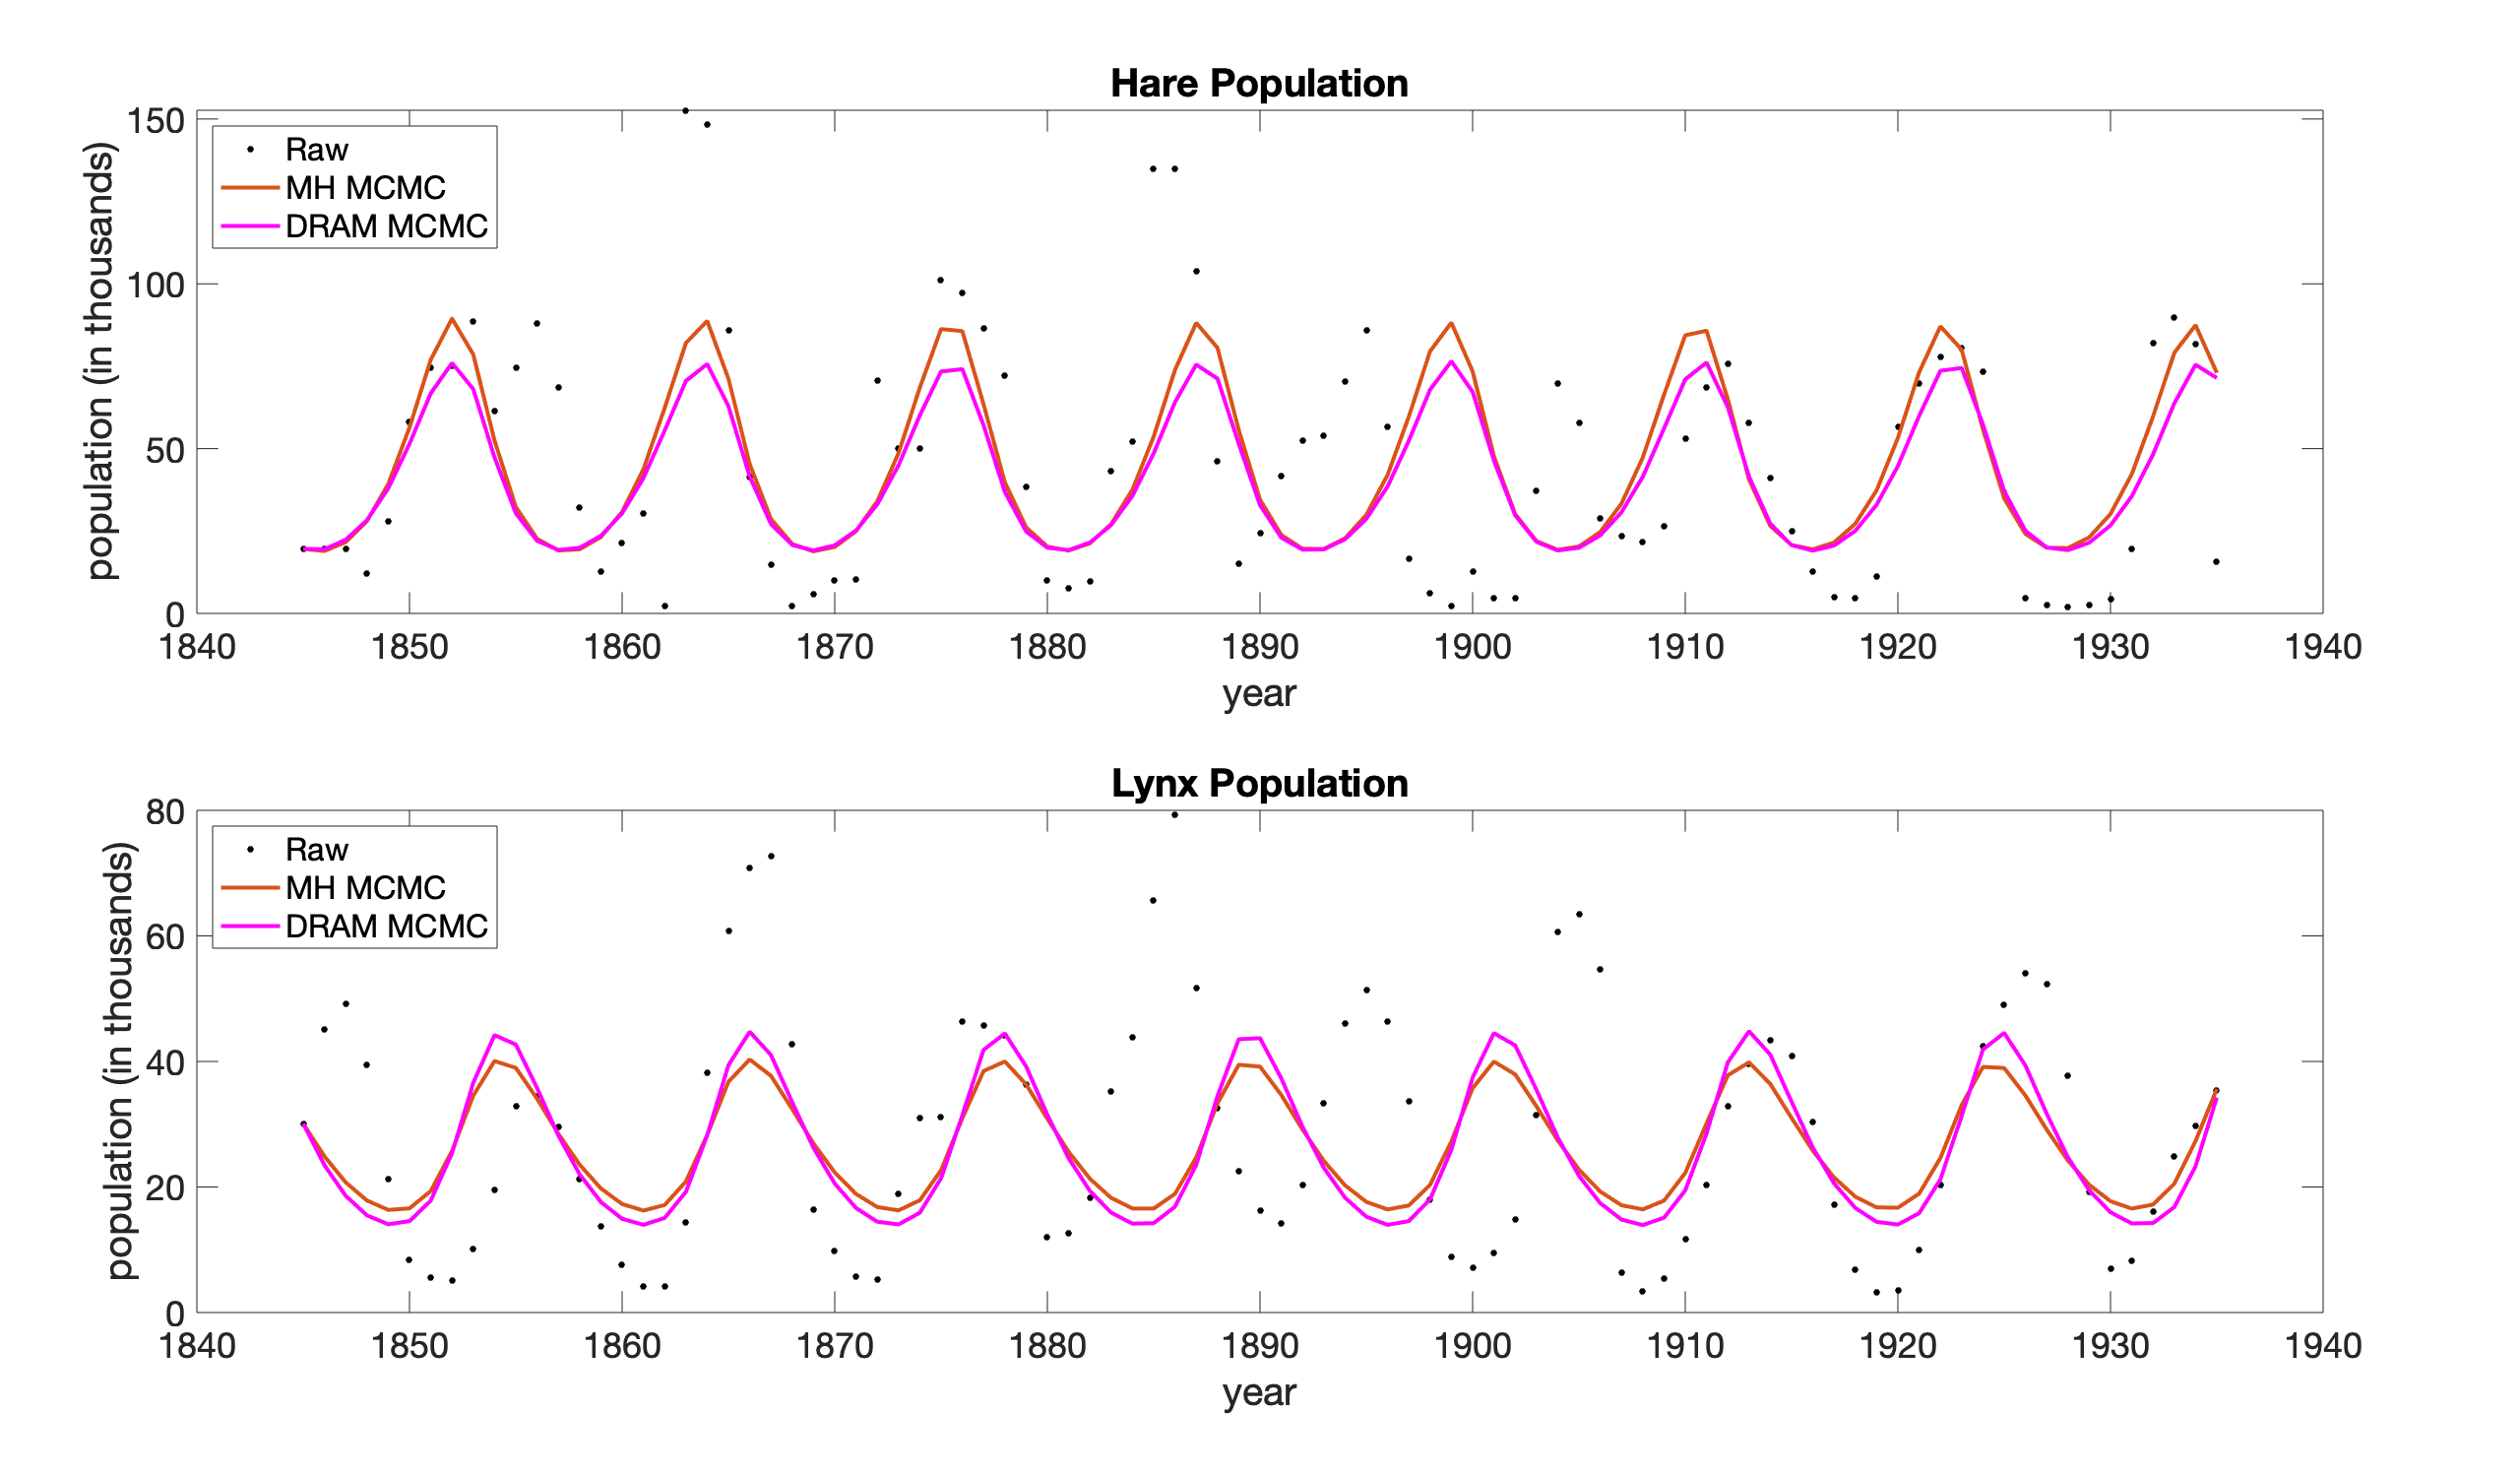
\includegraphics[width=15cm]{Final_Paper_Pieces/LV_Comparison_Figs/LVMCMC.png}
    \caption{Plot of raw mouse 6 data overlayed with MCMC, UKF, and PSO fits. It is evident that there is range of success on the individual mouse, with PSO appearing to perform best.}
    \label{fig:LVmcmc}
\end{figure}
As this figure illustrates, both MCMC methods are doing a fairly good job of capturing the periodic trends of both the hare and lynx populations as there seems to be similar periods between the original data and each algorithm. However, both algorithms struggle to capture the starting behavior for both populations, particularly the years 1840 to around 1900. Neither algorithm is able to capture the large spike in hare population around 1865. We next formally compare the two algorithms using RMSE scores.
\begin{table}[H]
\centering
        \begin{tabular}{c | c c}
            \cline{1-3}
            \textbf{MCMC Algorithm}  &\textbf{Hare} & \textbf{Lynx}\\
            \hline
            Metropolis & 18.16 & 31.30\\
            DRAM & 18.03 & 31.66
             \\\hline
            \hline
        \end{tabular}
    \caption{Formal comparison of the Metropolis and DRAM MCMC methods on the Lotka-Volterra system using root mean squared error (RMSE). Based on RMSE scores, there is no significant difference between the two predictions. We conclude that both are sufficiently predicting the original data for both populations.}
    \label{tab:LVmcmcpso}
\end{table}
Table \ref{tab:LVmcmcpso} confirms our hypothesis that both the Metropolis and DRAM algorithms are successfully capturing the orginal data for both the hare and lynx populations.
\par We next make a comparison between PSO algorithms using a log-likelihood objective function (PSO LL) and a sum of squares objective function (PSO SS).
\begin{figure}[H]
    \centering
    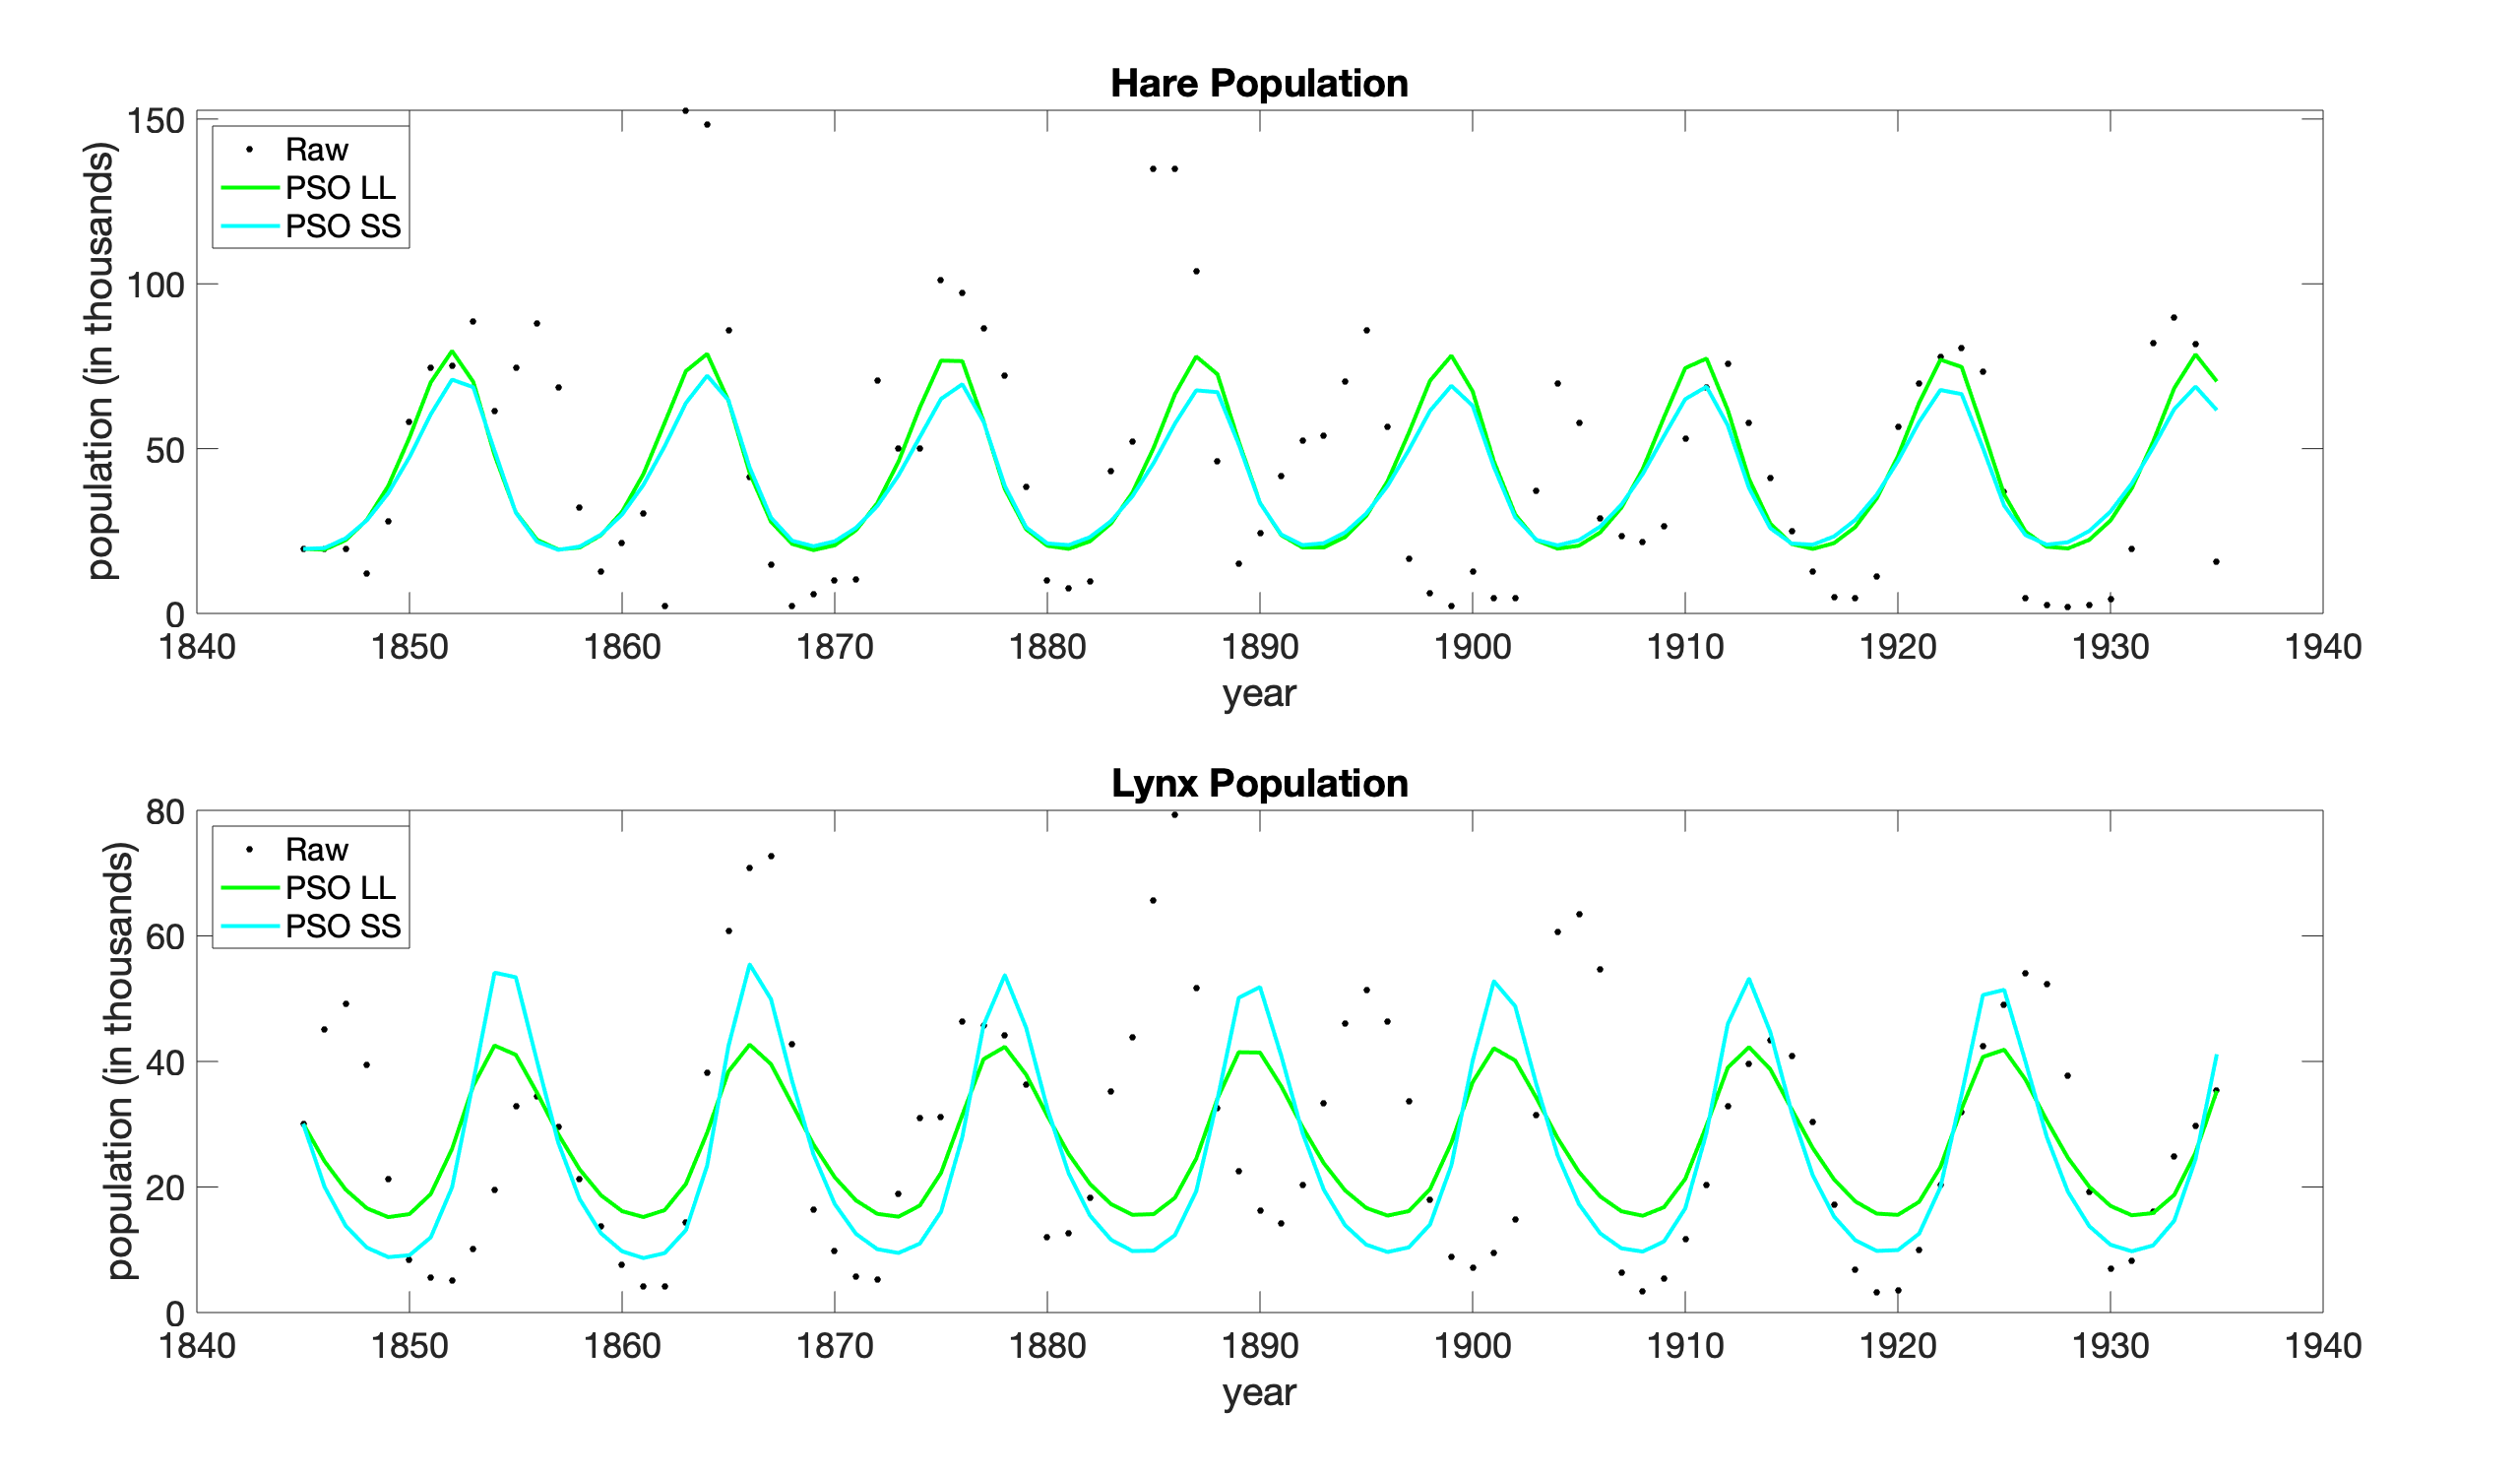
\includegraphics[width=15cm]{Final_Paper_Pieces/LV_Comparison_Figs/LVPSO.png}
    \caption{Plot of raw mouse 6 data overlayed with MCMC, UKF, and PSO fits. It is evident that there is range of success on the individual mouse, with PSO appearing to perform best.}
    \label{fig:LVpso}
\end{figure}
Like the MCMC methods, the PSO algorithms are both doing a good job of capturing the original data. Again, we see similar period between original data and each algorithm. In the lynx population, the PSO SS appears to capture more of the starting behavior as it has a greater amplitude, something that we do not see in the PSO LL or either of the MCMC methods. We next formally compare the two PSO algorithms using RMSE scores.
\begin{table}[H]
\centering
        \begin{tabular}{c | c c}
            \cline{1-3}
            \textbf{PSO Algorithm}  &\textbf{Hare} & \textbf{Lynx}\\
            \hline
            PSO LL & INSERT & INSERT \\
            PSO SS & INSERT & INSERT
             \\\hline
            \hline
        \end{tabular}
    \caption{Formal comparison of the PSO algorithms using a log-likelihood (PSO LL) and a sum of squares (PSO SS) objective function on the Lotka-Volterra system using root mean squared error (RMSE). FINISH ANALYSIS}
    \label{tab:LVpso}
\end{table}
***INSERT ANALYSIS OF TABLE
\par Finally we visually compare the population predictions from the Joint and Dual UKF parameterizations.
\begin{figure}[H]
    \centering
    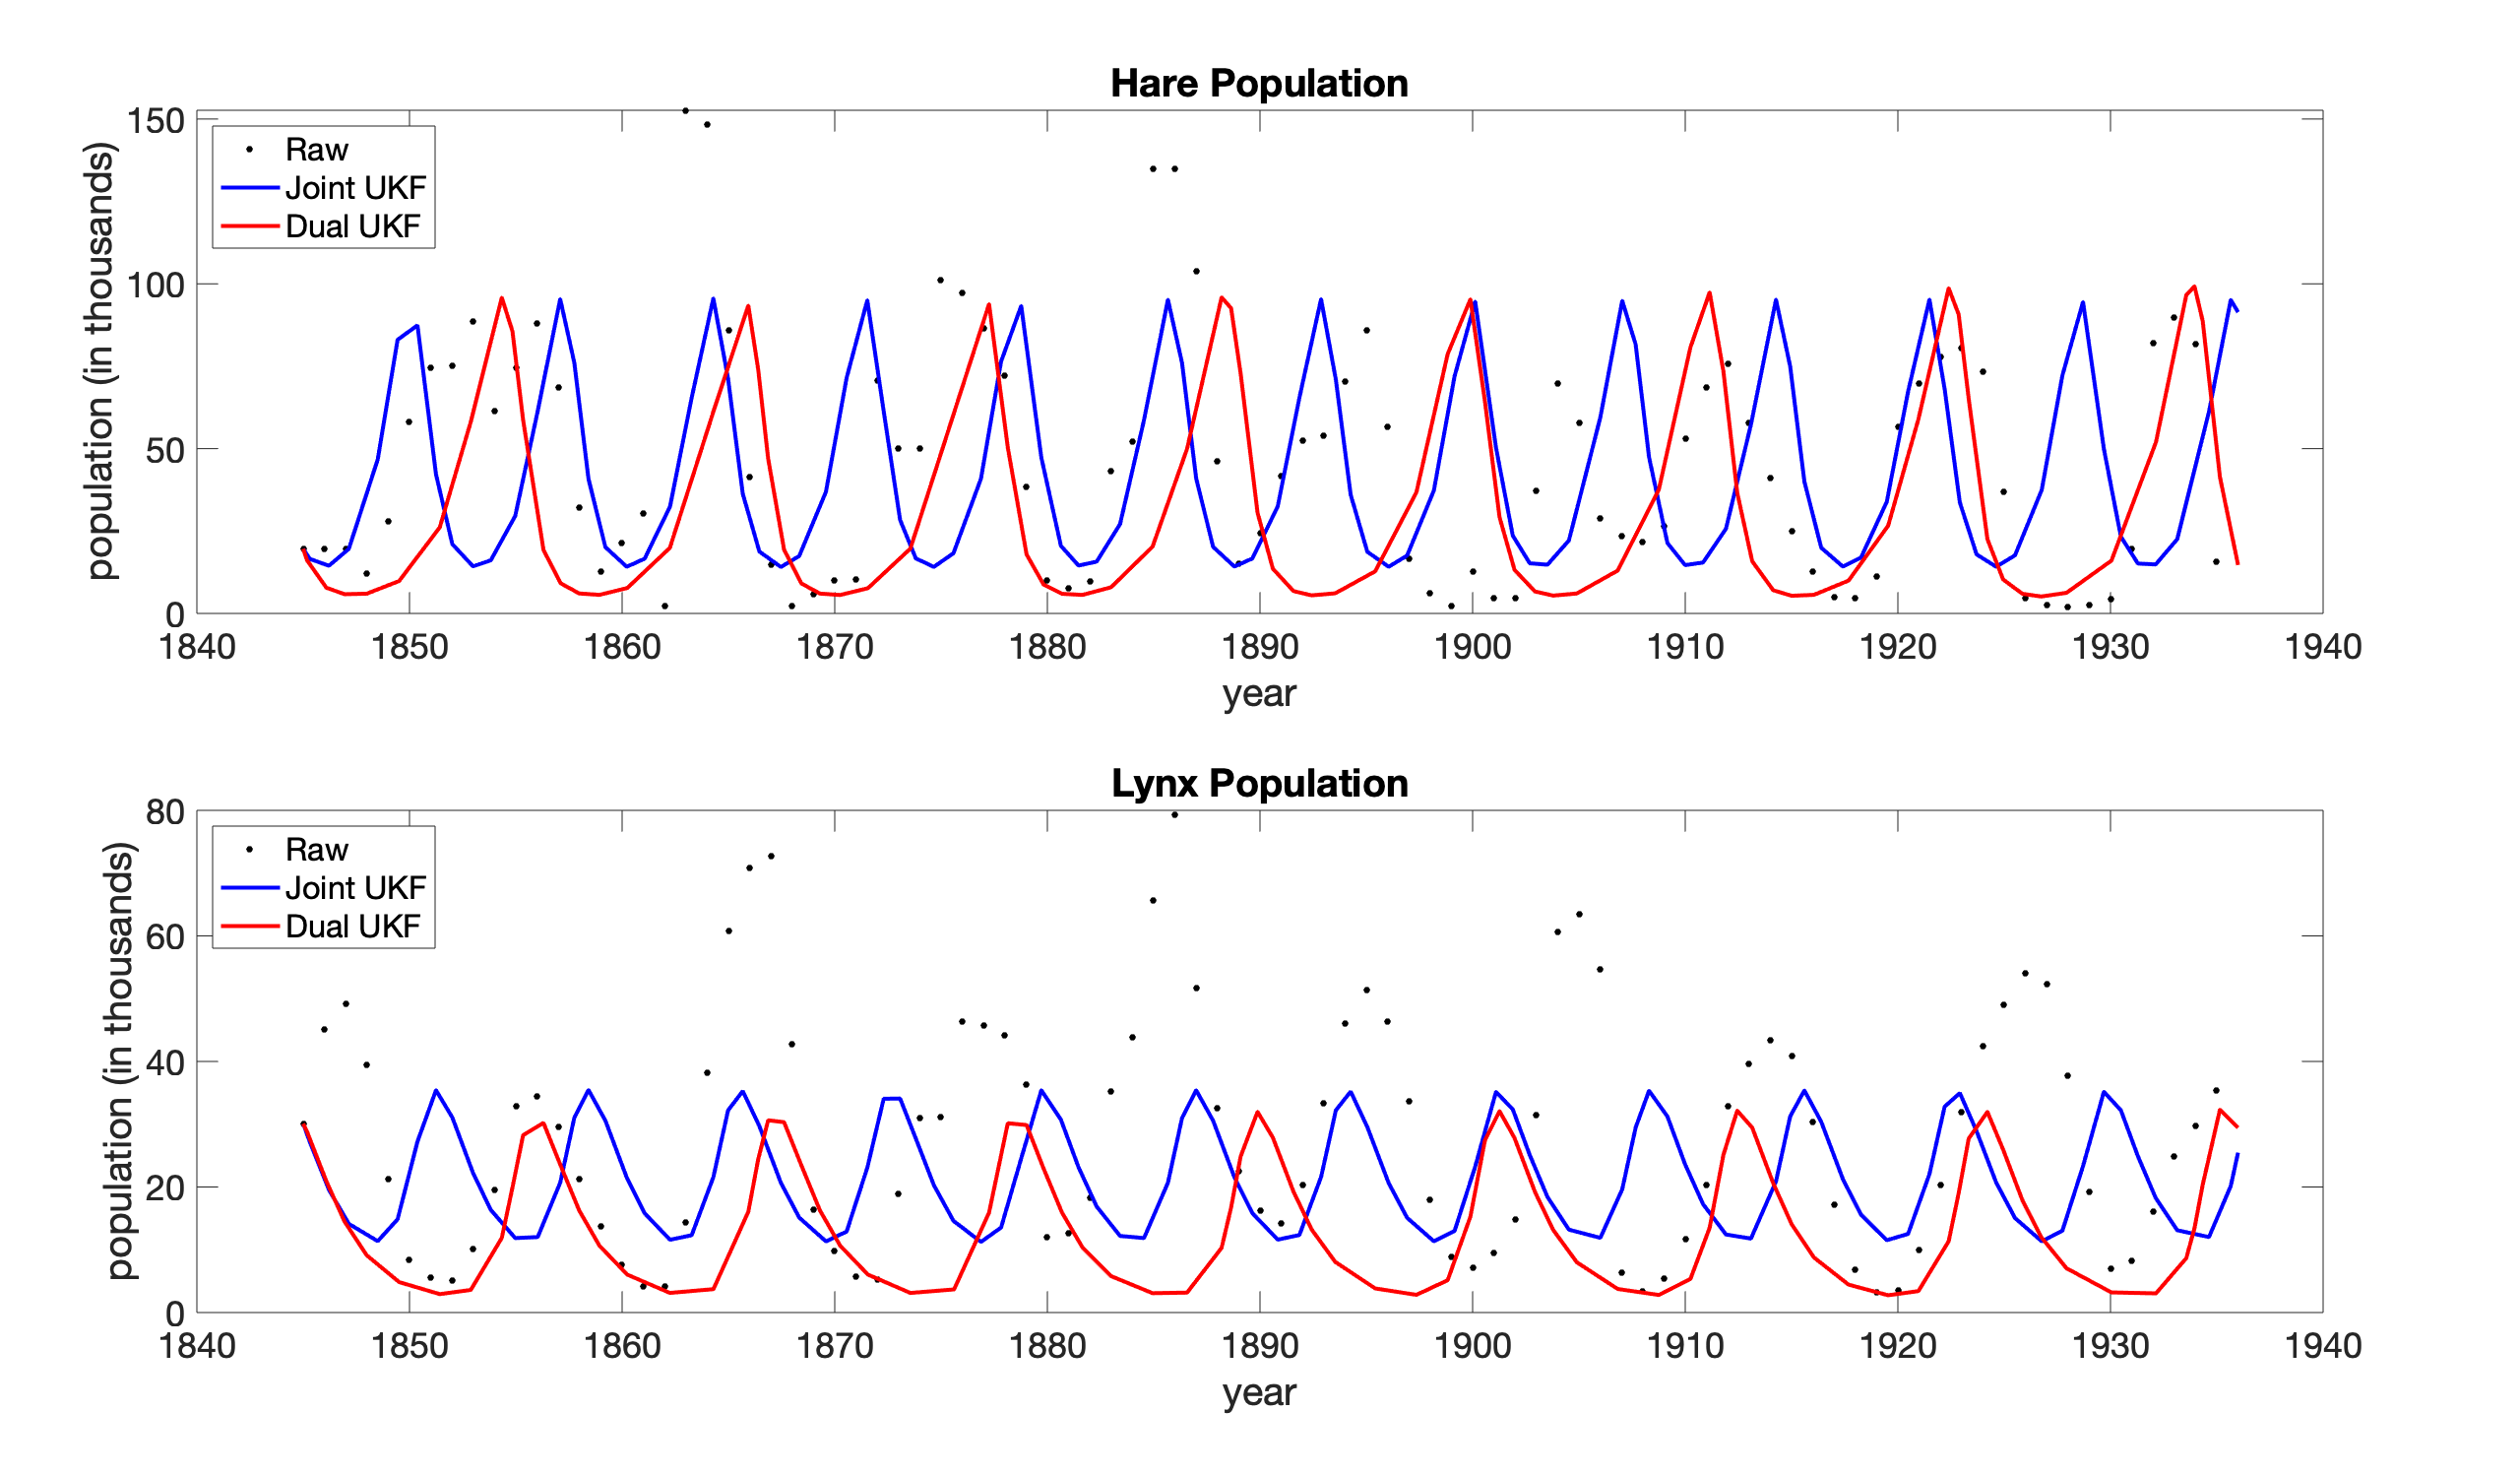
\includegraphics[width=15cm]{Final_Paper_Pieces/LV_Comparison_Figs/LVUKF.png}
    \caption{Plot of raw mouse 6 data overlayed with MCMC, UKF, and PSO fits. It is evident that there is range of success on the individual mouse, with PSO appearing to perform best.}
    \label{fig:LVukf}
\end{figure}
From Figure \ref{fig:LVukf} we can see that the UKF algorithms are doing a fair job of capturing the original data for both populations. These algorithm predictions differ from each other more drastically than we saw in either the MCMC or PSO predictions. The Joint UKF appears to have a shorter period than the original data while the Dual UKF has a similar period to the original data. In the lynx population, the Dual predicts a generally smaller population than the Joint, whereas in the hare population, the predictions were similar in size. We formally compare the predictions with RMSE scores.
\begin{table}[H]
  \begin{center}
    \begin{tabular}{c|c c} % <-- Alignments: 1st column left, 2nd middle and 3rd right, with vertical lines in between
      \hline
      \textbf{UKF Algorithm} & \textbf{Hare} & \textbf{Lynx} \\
      \hline
      \textbf{Joint} & 42.5392 & 22.2058\\
      \textbf{Dual} & 36.665 & 25.2749\\\hline
      \hline
    \end{tabular}
    \caption{Root Mean Squared Error (RMSE) of ODE simulations using final parameter values from Joint and Dual UKF's from Prey and Predator populations. As described in section \ref{section:DualUKF}, we consider the Dual to have better performance because of overall lower RMSE values and more realistic frequencies.}
    \label{table:Results_LV_ODESims_RMSE}
  \end{center}
\end{table}
In Table \ref{table:Results_LV_ODESims_RMSE} we can see that the Joint UKF seems to fit the lynx population better, while the Dual UKF does a better job on the hare population. As a whole, the Dual UKF seems to perform better than the Joint UKF.
\par Now that we have discussed individual algorithm performance of parameterizing the Lotka-Volterra system, we compare the best predictions from each algorithm. In Figure \ref{fig:LVall} we compare the PSO SS, DRAM MCMC, and Dual UKF algorithms.
\begin{figure}[H]
    \centering
    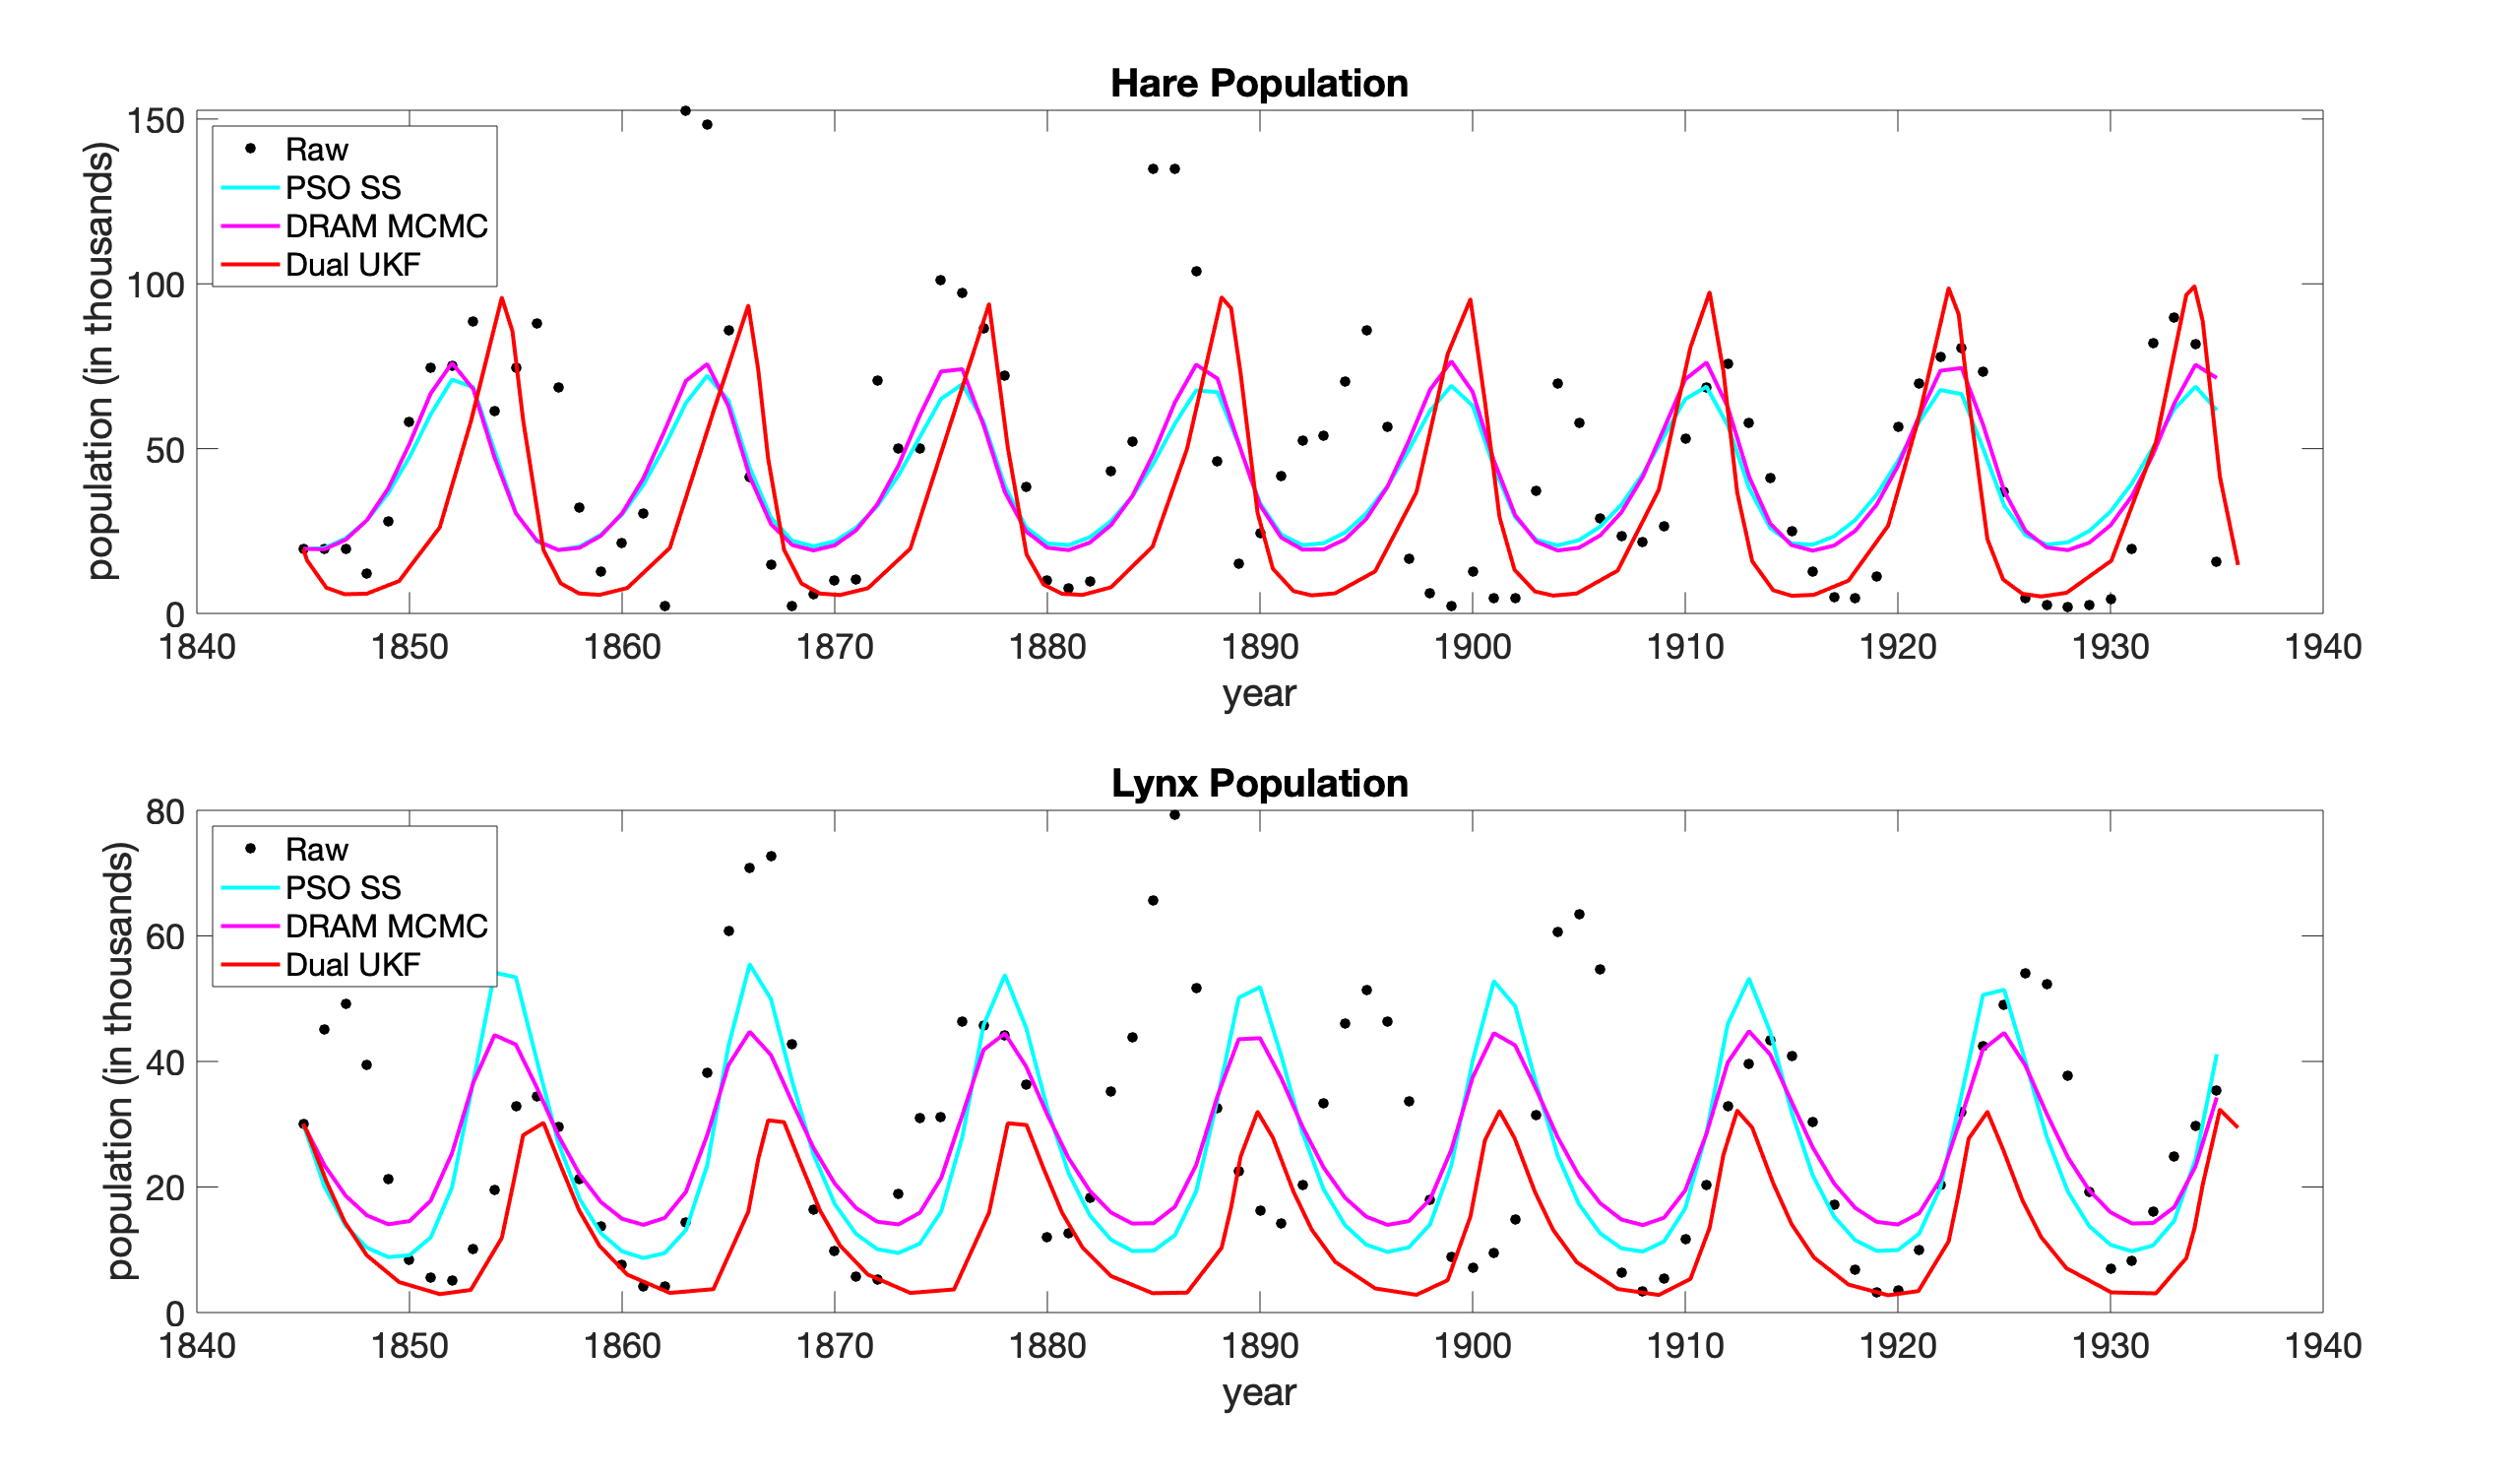
\includegraphics[width=15cm]{Final_Paper_Pieces/LV_Comparison_Figs/LVall_v2.png}
    \caption{Plot of raw mouse 6 data overlayed with MCMC, UKF, and PSO fits. It is evident that there is range of success on the individual mouse, with PSO appearing to perform best.}
    \label{fig:LVall}
\end{figure}
While all the algorithms did a fairly good job of capturing the original data, it is interesting to note the similarities and differences between predictions. We note that all three algorithms have periods similar to each other and to the original data. In the hare population, the PSO SS and DRAM MCMC predictions are the most similar particularly in amplitude and period. In the years 1840 to around 1890, the Dual UKF predition peaks higher and a little later than the other two algorithms. From 1900 to 1940, all three algorithms predict peaks in the hare population at the same time. In the lynx population prediction we note that all three algorithms have more similar periods than in the hare population. However, the PSO SS algorithm peaks the highest, the DRAM MCMC the second highest, and the Dual UKF has the lowest peak. It is interesting to see more difference in population levels particularly between the PSO SS and DRAM MCMC methods which were much more similar in the hare population prediction. Overall, we believe all three algorithms have performed well and captured the original data. We compile their respective RMSE scores for a final formal comparison.
\begin{table}[H]
\centering
        \begin{tabular}{c | c c}
            \cline{1-3}
            \textbf{Algorithm}  &\textbf{Hare} & \textbf{Lynx}\\
            \hline
            PSO SS & INSERT & INSERT \\
            DRAM MCMC & 18.03 & 31.66\\
            Dual UKF & 36.665 & 25.2749\\\hline
            \hline
        \end{tabular}
    \caption{Formal comparison of the PSO algorithm using a sum of squares (PSO SS) objective function, the DRAM MCMC algorithm, and the Dual UKF on the Lotka-Volterra system using root mean squared error (RMSE). FINISH ANALYSIS}
    \label{tab:LVdrampsoukf}
\end{table}
% FINISH ANALYSIS WITH PSO RMSE IN


\subsection{Type 1 Diabetes}

\subsubsection{Approach To Comparisons}

In the context of the T1D model, we will compare the MCMC, UKF, and PSO approaches on both a population and individual level. Recall that for the T1D Model we use data from 11 different mice, 9 of which we classified as acute and 2 of which we classified as progressive as in Section \ref{section:T1D_individual_data}. For our population comparison, we will show fits done on an average of all the data from the acute mice, and for the individual level comparison, we will compare fits done on Mouse 6. We choose to compare the algorithms' performances in two different contexts in order to gain an understanding of the algorithms' performance in various situations. We hope that this will allow us to determine when a certain algorithm would be preferable over its counterparts.


\subsubsection{Individual Level Comparison}
To perform an individual-level comparison, we utilize mouse 6 as an example. As explained when utilized by the UKF algorithms, mouse 6 has been determined in an ad hoc fashion to be a good representation of the population as a whole as it provides us with 10 raw data points, significantly more than the average of 6.91. To get the Kalman Filter fits we use the standard approach used thus far of performing five iterations and choosing the best based on MSE value. Next, for MCMC we now run the algorithm using \emph{just} mouse 6 data, instead of the averaged Li data as was done previously. Finally, for PSO we run the algorithm, just as with MCMC, on the mouse 6 data only. To assess quality of fit, we use the same visual and numerical criteria of plotting fits and considering RMSE values as before. 
\begin{figure}[H]
    \centering
    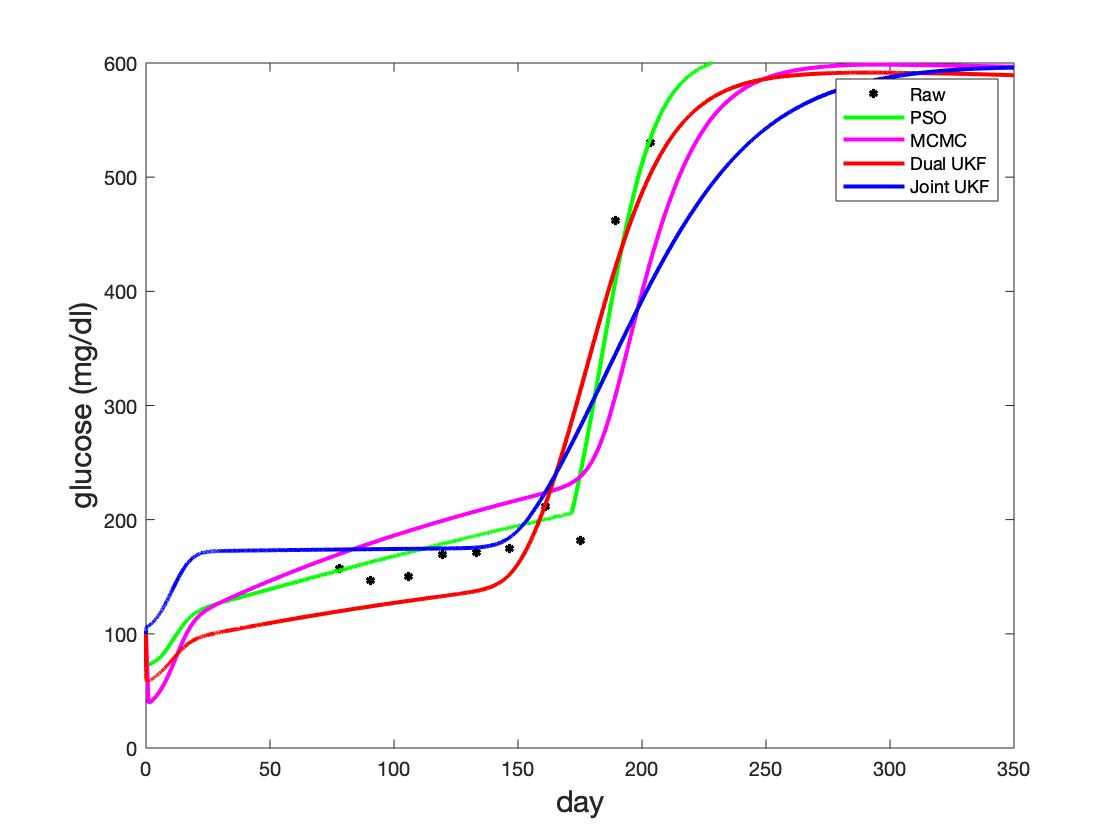
\includegraphics[width=15cm]{Comparison_Figures/Mouse6_ComparisonFigure_AllAlgorithms.jpg}
    \caption{Plot of raw mouse 6 data overlayed with MCMC, UKF, and PSO fits. It is evident that there is range of success on the individual mouse, with PSO appearing to perform best.}
    \label{fig:Results_Mouse6_Comparison}
\end{figure}
Visually, as seen in Figure \ref{fig:Results_Mouse6_Comparison}, it is reassuring to see that we achieve similar results across the 4 algorithms. We mean this in the sense that every algorithm follows a similar shape and appears to predict similar onset times. However, we do see a difference in starting behavior where the PSO, MCMC, and Dual UKF all start with glucose around 100 $\frac{mg}{dL}$ then show a decrease before the slow steady increase, while the Joint UKF immediately begins its increase. Interestingly, it appears that after increasing to glucose of around 175 $\frac{mg}{dL}$, the prediction levels off or possibly even decreases very slightly until it reaches its pivot point. Overall, we see visually that the PSO algorithm appears to fit the raw data the best. However, there is an odd angle occurring at the pivot point in the PSO prediction. This should be a smooth curve as the others illustrate and it is not quite clear to us what is causing this angle. Despite this odd shape, we again use the root mean squared error of each algorithm to score performance.
\begin{table}[H]
  \begin{center}
    \begin{tabular}{c|c} % <-- Alignments: 1st column left, 2nd middle and 3rd right, with vertical lines in between
      \textbf{Algorithm} & \textbf{RMSE} \\
      \hline
      \textbf{PSO} & 28.2\\
      \textbf{MCMC} & 66.8\\
      \textbf{Dual UKF} & 50.2\\
      \textbf{Joint UKF} & 67.1
    \end{tabular}
    \caption{Root Mean Squared Error (RMSE) of ODE simulations using parameter estimates to fit to Li mouse 6 data. The quantification of the error confirms our visual hypothesis that PSO performs the best fit on this data set.}
    \label{table:Results_Mouse6_RMSE}
  \end{center}
\end{table}
Table \ref{table:Results_Mouse6_RMSE} confirms that the PSO algorithm is indeed fitting the raw data the best. We note that the Dual UKF is outperforming the MCMC algorithm and while the MCMC scores better than the Joint UKF method, the two scores are very similar. This also lends support to our assertion that the Dual UKF normally outperforms the Joint UKF, as well as that the PSO is versatile in the datasets it may be applied to. 


\subsubsection{Population Level Comparisons}

\paragraph{Comparison of Averaging Techniques}
The averaged version of the Li et al dataset was produced as in Section \ref{section:T1D_population_data} in order to understand the predicted behavior of a general mouse in the cohort. In dealing with the average data, we consider two approaches to fitting this dataset:
\begin{enumerate}
    \item Average Then Fit: Run algorithm on the already averaged dataset.
    \item Fit Then Average: Run algorithm on each mouse individually and then average the parameter values
\end{enumerate}
In the first scenario, we treat the averaged data as a new dataset, as was done in the for the traditional MCMC fits. However, in our second option, we fit to every mouse individually, as was performed in the UKF section \ref{section:UKF_T1D_Implementation} and then treat averages of those parameters as the new final parameters. For example, a parameter value for $G_I$ is found for every mouse, and then the mean of these values is used to understand the population. Thus, in this case the algorithms never work with the averaged dataset directly. We chose to test both approaches since the UKF has not historically been used with averaged data. As a result, we are not initially sure which approach would work best and thus attempt both to allow us to know in the future how best to deal with averaged data. First, let's consider scenario one on the MCMC and PSO algorithms. This represents the standard way one would use averaged data as has been done throughout the paper thus far.


%{In order to compare the algorithms at a population level, we use average acute mice data as prepared in section X. Then, we produce the following four fits to this data. First, we use the mean parameters from the MCMC posterior distributions achieved from running the algorithm on this data set. Next, the second and third fits come from averaging the final parameter values achieved on the set of acute mice from the Joint and Dual UKF algorithms. For example, a final value of $\eta$ was produced by running the algorithms on each mouse. Now, we average all of those $\eta$ values to produce a population-level parameter. Our fourth fit is from running the PSO on the population level data. In order to assess the goodness of fit, we plot the fits on top of one another along with the raw data for a visual check and also compare the MSE values. %}


\paragraph{Average First with MCMC and PSO}
\begin{figure}[H]
    \centering
    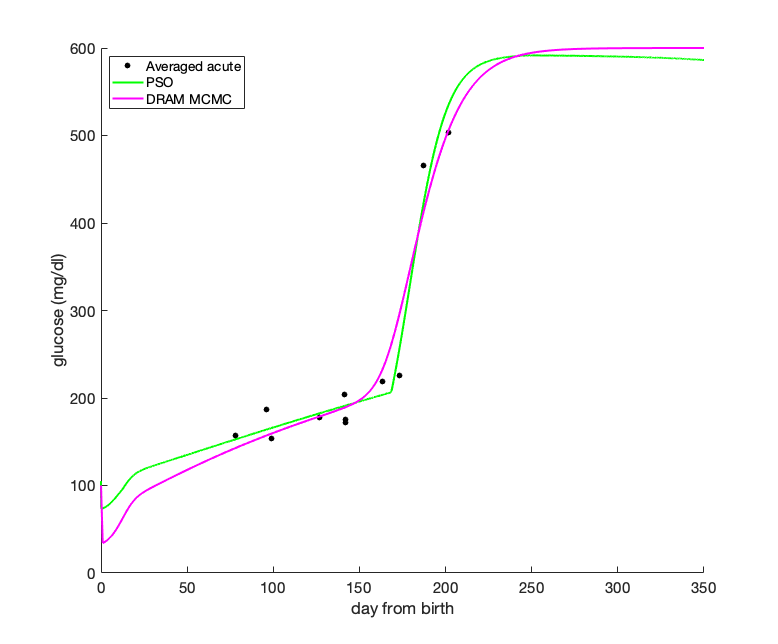
\includegraphics[width=15cm]{Comparison_Figures/averagethenfit_pso_dram_comp.png}
    \caption{Plot of averaged acute Li data overlayed with PSO and DRAM MCMC fits. This figure illustrates the results of averaging data then fitting. Both predictions are doing a good job of capturing the general trend of the average data. It is difficult to determine by eye which algoirthm is performing the best.}
    \label{fig:Results_Averaged_PSOMCMC_Fit}
\end{figure}
From Figure \ref{fig:Results_Averaged_PSOMCMC_Fit}, both algorithms are doing a fair job of capturing the raw averaged data. We are unsurprised at the goodness of fit from the DRAM MCMC algorithm as many studies utilize MCMC methods to parameterize on large often averaged data sets. The PSO fit provides us with a loose validation that averaging data before parameterizing does indeed produce satisfactory results. We look to the root mean squared error scores to provide us with more comparative information between algorithms.
\begin{table}[H]
  \begin{center}
    \begin{tabular}{c|c} % <-- Alignments: 1st column left, 2nd middle and 3rd right, with vertical lines in between
      \textbf{Algorithm} & \textbf{RMSE} \\
      \hline
      \textbf{PSO} & 22.75\\
      \textbf{DRAM MCMC} & 30.71\\
    \end{tabular}
    \caption{Root Mean Squared Error (RMSE) of ODE simulations using PSO and DRAM MCMC. Each algorithm was run on pre-averaged acute data. The RMSE scores tell us that the PSO has performed marginally better than the DRAM MCMC, however both are doing a satisfactory job of capturing the data.}
  \end{center}
  \label{tab:mcmcpsoT1D}
\end{table}
While the root MSE tells us that the DRAM MCMC algorithm performed slightly better than the PSO method, the scores are not significantly different. While not a perfect fit of the data, we are satisfied that both algorithms have performed well. These results help us to confirm that averaging data before parameterization is a good method for producing biologically feasible results.
\subsubsection{Average First verus Fit First}
UKF algorithms have traditionally been used on individual-level data. Thus, there are no established techniques from literature for how to utilize averaged data. One obvious approach is option 1. However, due to our hypothesis that UKF's are better suited for option 2, we thus attempt to perform the fit this way as well. Once again, we use the PSO as a tool for comparison. In Figure \ref{fig:T1D_Results_AveragingTechniques_Comparison}, we present plots demonstrating the difference in fits for the Joint UKF, Dual UKF, and PSO when using option 1 versus option 2. Additionally, we compare all of the fit first results in the final panel, as performing individual fits is the context in which he have used the UKF's the most.

\begin{figure}[H] 
    \centering
    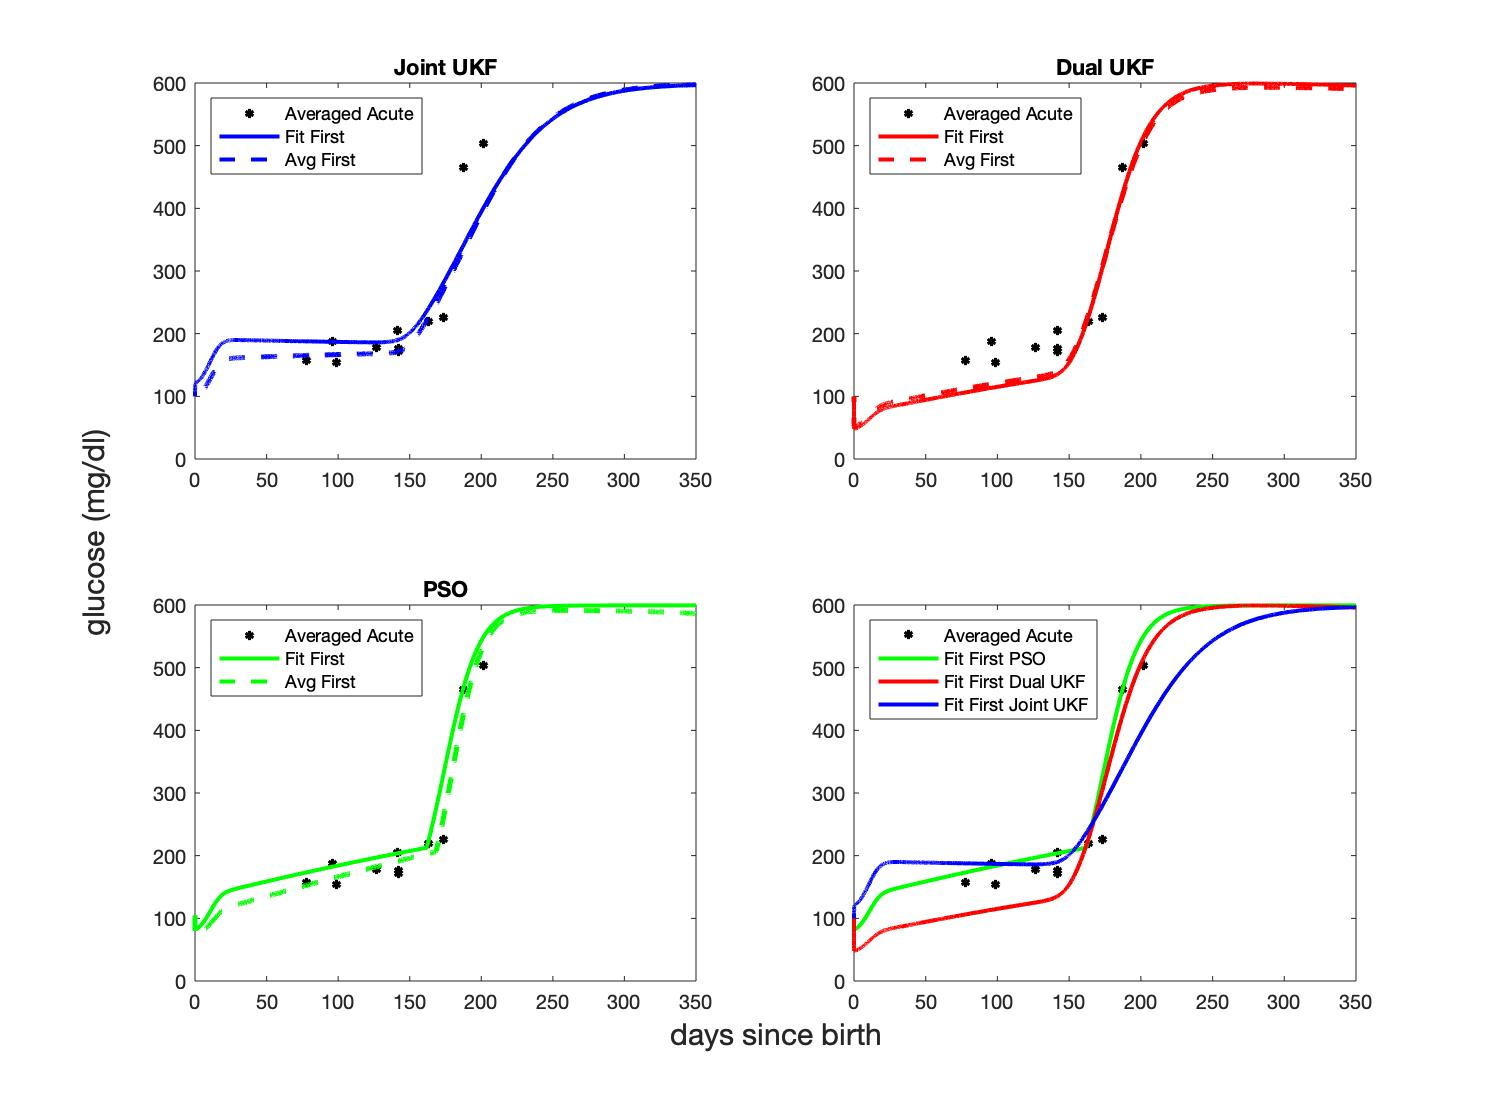
\includegraphics[width=20cm]{Comparison_Figures/T1D_AveragingTechniques_PSOUKF_New.jpg}
    \caption{Plots of using Joint and Dual UKFs, as well as PSO, to fit to averaged Li data by both running the algorithms directly on this dataset as well as by averaging parameters from individual fits instead of training on the actual averaged dataset. It is evident that averaging first produces slightly better results for PSO and the Joint UKF. For the Dual UKF, the fits are so similar it is hard to see which is better. Additionally, we compare the Fit First results in the final subplot to demonstrate the PSO's superior performance here.}
    \label{fig:T1D_Results_AveragingTechniques_Comparison}
\end{figure}
Looking at the PSO fits first, the difference in technique does not appear to alter results significantly. A slight advantage is seen in averaging first, however by no means a drastic one. This is corroborated by both the Joint and Dual UKF fits. Thus, it appears that if one's intention is to work with averaged data, training directly on the averaged data may provide a slight advantage, but there is overall little difference. More importantly, as compared to the UKF fits in section \ref{section:T1D_DualUKF_Results} which were performed on data from a single mouse, the performance here appears worse. This confirms our hypothesis that UKF's perform better on individual-level data, and we will soon see a potentially more effective way to incorporate UKF methods as part of a fit to averaged data in section \ref{Combining_UKF_MCMC}. Finally, in our fourth panel it is evident that the PSO performs best overall. This is confirmed through an analysis of RMSE values for these fits in Table \ref{table:Results_FitFirst_RMSE}.


\begin{table}[H]
  \begin{center}
    \begin{tabular}{c|c} % <-- Alignments: 1st column left, 2nd middle and 3rd right, with vertical lines in between
      \textbf{Algorithm} & \textbf{RMSE} \\
      \hline
      \textbf{PSO} & 35.46\\
      \textbf{Dual UKF} & 51.06\\
      \textbf{Joint UKF} & 52.07
    \end{tabular}
    \caption{Root Mean Squared Error (RMSE) of ODE simulations using a Fit First technique to capture averaged data. It is evident that the UKFs before similarly to each other but struggle as compared to the PSO.}
    \label{table:Results_FitFirst_RMSE}
  \end{center}
\end{table}
Both visually and numerically, it is evident that PSO performs best on this dataset. Overall, this analysis suggests that using UKF's directly on averaged data, whether by fitting first or averaging first, is most likely not an optimal approach. 

\subsection{Biological Feasibility} \label{Results_Biological_Feasibility}
So far we have focused our assessments of algorithm performance on predictions of glucose. However, the Type 1 diabetes model has other populations of cells that depend on glucose levels and on which glucose levels are also dependent \cite{shtylla2019mathematical}. Therefore a more comprehensive evaluation of the performance of our algorithms must consider the 11 other states within the ODE system. For a full list of these states and their equations see Appendix/Section X. We want to confirm that the parameters that our algorithms produce, in addition to generating biologically viable glucose predictions, will also generate biologically viable predictions for other states.  In the following sections for each algorithm we will compare predictions of 4 states from the T1D ODE system with pre-parameterized evaluations of the T1D ODE system, that is using baseline parameter values. The 4 states we analyze are Apoptotic beta cells, Insulin, Effector T cells, and Regulatory T cells. These states capture both the similarities and differences between the baseline and final parameters, however a similar comparison for all 12 states can be found in Appendix \ref{general_appendix}. 
\par In addition to this visual assessment of biological feasibility, we do a final evaluation of each algorithm's performance by assessing the ability of the algorithm to predict diabetes onset. In the ODE model, we can turn the apoptotic $\beta$-cell wave on and off. With the wave on, the mouse should develop diabetes and without the wave, the mouse should not. Each of the algorithms have been parameterized on the ODE model with the wave on. We parameterize with the wave because we are working with data in which the mice have been shown to develop diabetes, therefore we want our model to reflect the onset. However, the parameters produced during these parameterizations would ideally be sensitive to the presence or absence of the apoptotic $\beta$-cell wave. That is, by simply evaluating our model without the wave, we should be able to predict glucose levels for a mouse that does not develop diabetes using the final parameter values from each algorithm. We will explore this idea in Section \ref{NoWaveModels}.
\subsubsection{DRAM MCMC} \label{biocheck_dram}
Figure \ref{fig:dram_biocheck} compares the state predictions using mean parameter values fitted using the DRAM parameterization performed on Mouse 6 data with the pre-parameterized evaluation of the T1D ODE system using baseline parameter values.
\begin{figure}[H] 
    \centering
    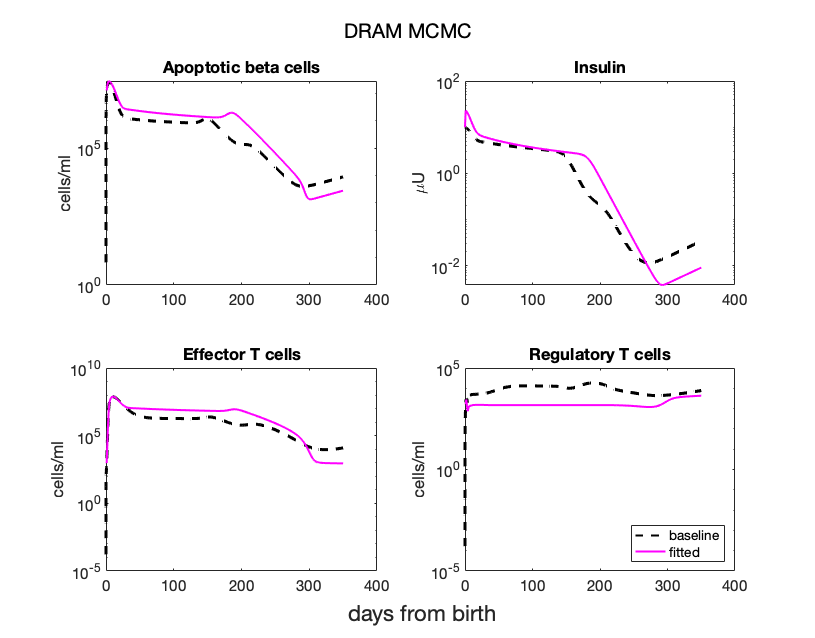
\includegraphics[width=15cm]{MCMC_figs/dram_t1d_final/mouse6_importantStates.png}
    \caption{State predictions using parameter values fitted using the DRAM parameterization on Mouse 6 data. Predictions are plotted in magenta and the dashed line indicates the baseline, pre-parameterized evaluation of the particular state. The DRAM algorithm produces biologically feasible results for all four states evaluated.}
    \label{fig:dram_biocheck}
\end{figure}
This figures indicates that the DRAM MCMC parameterization produces biologically feasible results. Therefore we can be more confident in using the final parameter values. Although the initial behavior of each DRAM predictions differ from those of the baseline, we are pleased to see that we can produce biologically feasible results for each state and that the predictions appear to be very similar to the baseline evaluations. 
\subsubsection{PSO}
Figure \ref{fig:PSO_biocheck} compares the state predictions given by PSO for Mouse 6 with the evaluation of the T1D model using baseline parameter values.
\begin{figure}[H] 
    \centering
    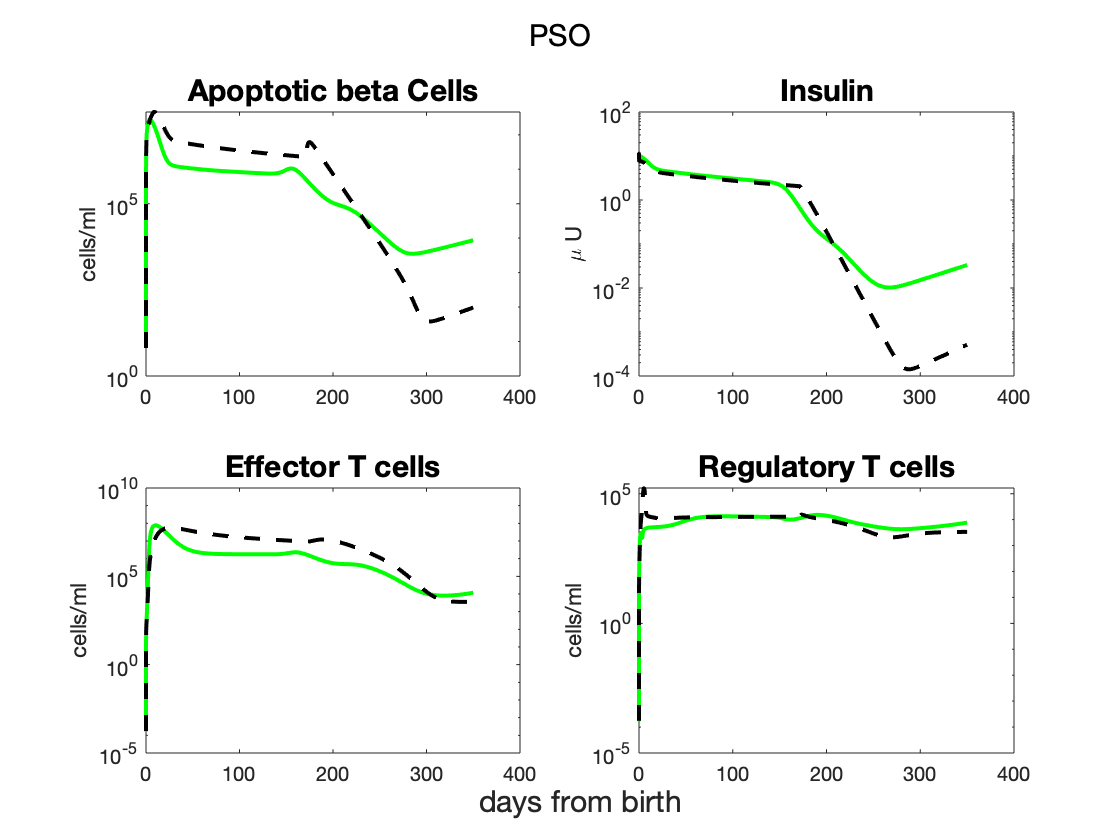
\includegraphics[width=15cm]{Final_Paper_Pieces/PSO_figs/PSO_biocheck.png}
    \caption{State predictions using parameter values fit using the PSO on Mouse 6 data. Predictions are plotted in green and the dashed line indicates the baseline evaluation, one that is known to be biologically feasible. PSO appears successful in capturing the general behavior of the states in question, but notably predicts less extreme behavior in the apoptotic beta cell population in comparison to the baseline, as well as a less intense dip in insulin around day 300.}
    \label{fig:PSO_biocheck}
\end{figure}
Though there is no formal threshold for determining whether a fit 'passes' the biological feasibility checks, the shapes of the state curves produced by PSO are very similar to that of the baseline parameters, known to be feasible.
\par First examining the apoptotic beta cells, both the PSO and baseline parameters produce large initial spikes. The PSO-predicted system reaches a slightly lower maximum than the baseline at a marginally earlier time. This is in keeping with the tendency of PSO to 'shift' the behavior of the baseline system earlier in time, as seen previously by the earlier onset time in the glucose prediction. A secondary spike is also seen in both the baseline and predicted system, however, again, this spike occurs earlier in the predicted system. Finally, a drop in apoptotic beta cells at approximately day 200 is seen in both simulations. The slope of this drop is gentler in the predicted system and does not reach as low of a minimum. This is the main notable difference in the apoptotic beta cell populations. 
\par The insulin curves of the two simulations mirror each other well in shape. They initially experience the same minor decrease from day 0 to approximately day 50, at which point the begin to decrease linearly with an almost identical slope. However, slightly prior to day 200, both simulations produce a linear drop of greater magnitude. This drop in the PSO-predicted system predates that in the baseline system, further evidencing the tendency of the PSO-predicted system to 'shift' behaviors earlier. It is unknown if this shift is a function of the data set, or of the parameterization method. Finally, the minimum insulin level reached by the PSO-predicted system is 2 orders of magnitude higher than that predicted by the baseline system. After reaching this minimum, however, both systems seem to rebound with similar slope.  
\par Finally, the Effector T cell and Regulatory T cell populations offer excellent fits. Not only does PSO capture the shape of the baseline, but also the timings and magnitudes of peaks. This suggests that the parameters involved in T cell interaction are likely reasonable. $\mu_e$ and $\mu_r$, two parameters involved, are known to be parameters of interest according to the notable parameter set discussed in Section 2, so it is exciting to see results that seem feasible from these sensitive parameters. 
\par To conclude, it is reassuring to see that PSO produces behavior that mimics that of the baseline system. This means that we can reasonably hypothesize that PSO produces parameters that would, in fact, describe pancreatic cell behavior within mouse 6, given the presence of the apoptotic wave. Especially due to the relatively large range of values
allowed in each parameter, this result becomes all the more exciting. 
\subsubsection{UKF}

First we have the results for the Dual in Figure \ref{fig:T1D_UKF_StateSubsets_WithWave}, displaying the 4 chosen states as predicted using parameters from the Dual UKF on mouse 6 compared to the baseline state predictions.
\begin{figure}[H] 
    \centering
    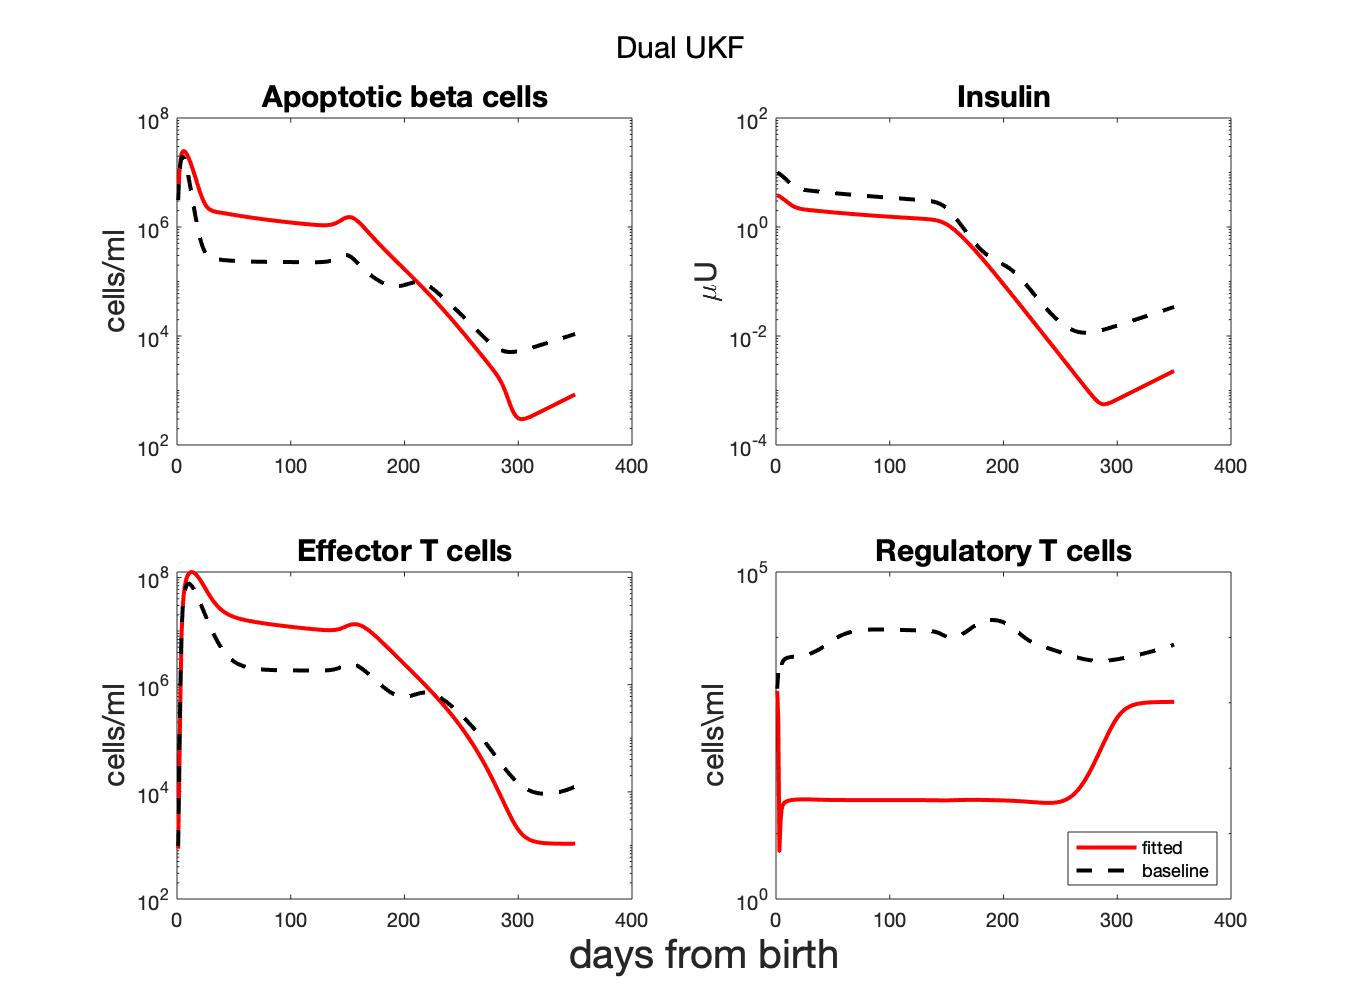
\includegraphics[width=15cm]{Kalman_Filter_Images/T1D_StateSubsets_DualBaselineOverlay.jpg}
    \caption{State predictions using parameter values fitted using the Dual UKF parameterization on Mouse 6 data. Predictions are plotted in red and the dashed line indicates the baseline, pre-parameterized evaluation of the particular state. We see that, although the results appear feasible in terms of their values, the trajectories are often smoothed out as compared to the baseline. We are particularly interested in the behavior of the Regulatory T cells here.}
    \label{fig:T1D_UKF_StateSubsets_WithWave}
\end{figure}
First off, it is assuring to see that none of our predicted states do anything extremely outlandish. The main difference we see between the Dual and Baseline results is in the Regulatory T Cells. With baseline parameters the Regulatory T Cells follow more of a curved path, while under the Dual estimates they flat line relatively early. A main parameter that controls the Regulatory, as well as Effector, T cells is their rates of interaction $\mu_e$ and $\mu_r$. In simplest terms, these control how good each type of T cell is at killing off the other. In the current set up, these are two separate parameters. However, in the baseline they are set to be equivalent. One idea we tried was thus to treat them as a single parameter in our UKF, however this unfortunately, and surprisingly, resulted in nearly identical results. Thus, T cell behavior continues to be one of the aspects needed to be explored further. Of course, there is a possibility that the results from the parameter estimate are actually feasible, however this could not be confirmed without raw T cell data. Additionally, the results from the final parameter estimates produce much smoother curves. This, most likely, is inaccurate and must be explored further as well.\\


%Figure

%Explanation

Now, we have the results for the Joint in Figure \ref{fig:joint_biocheck}

\begin{figure}[H] 
    \centering
    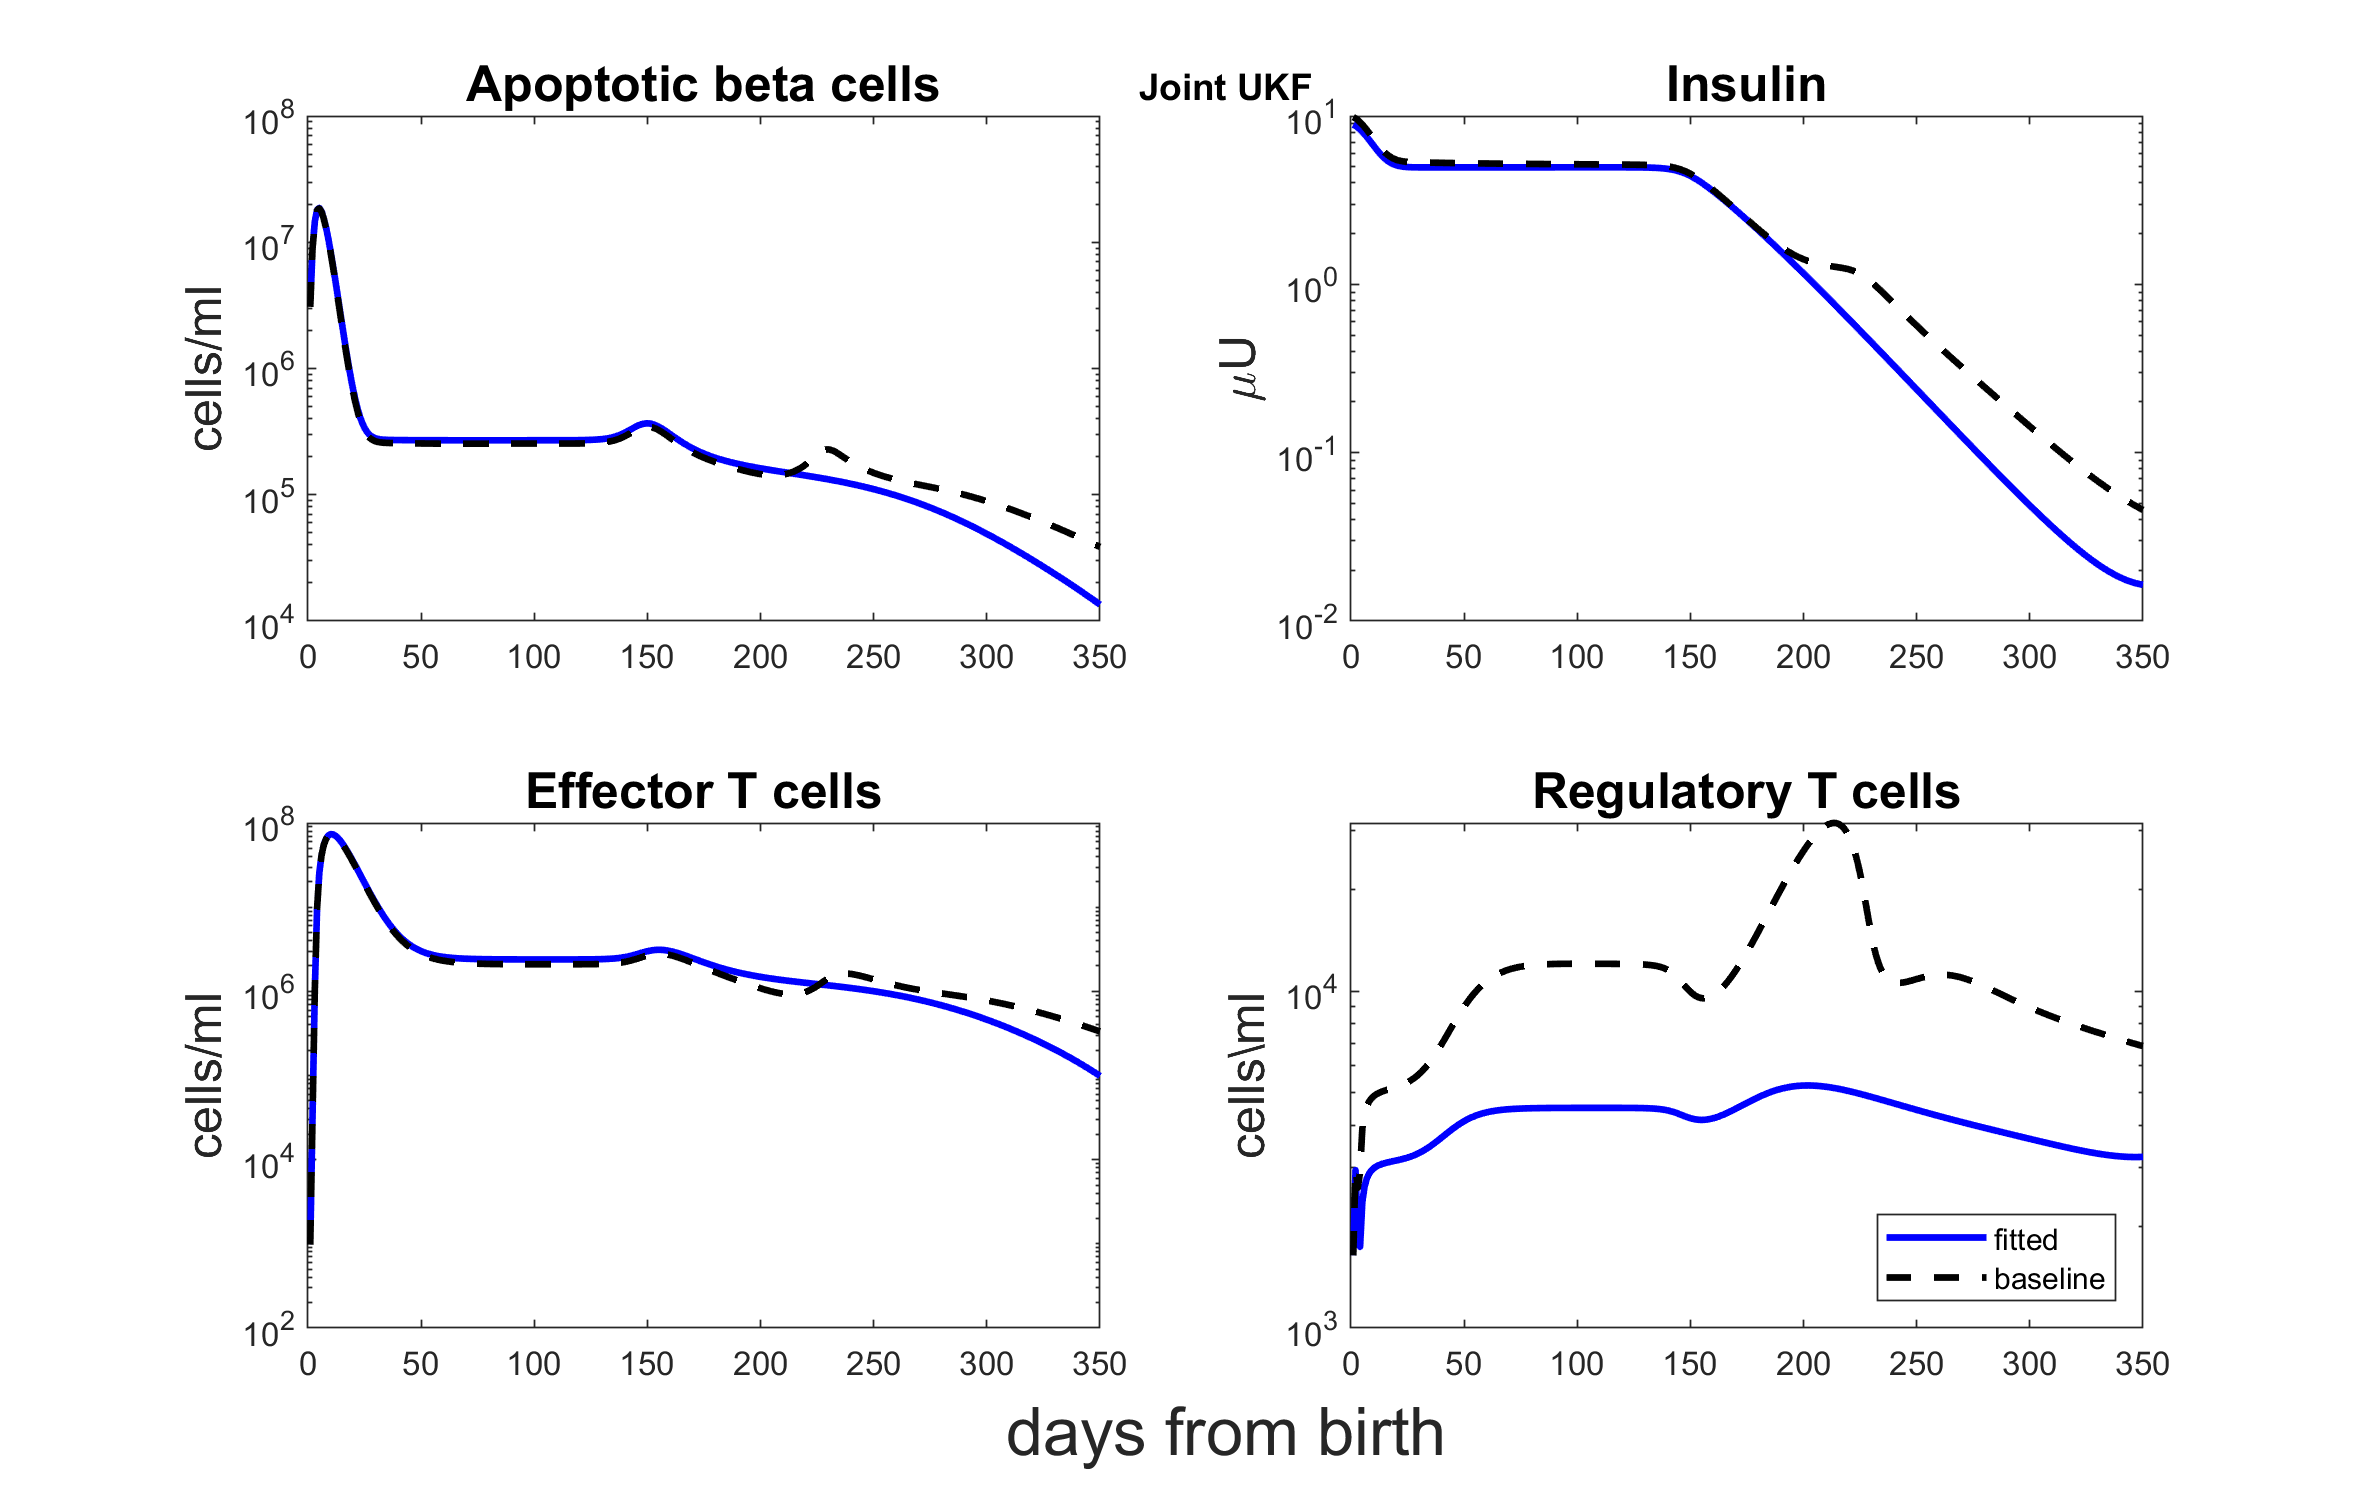
\includegraphics[width=15cm]{Kalman_Filter_Images/joint_mouse6_subsetofstates.png}
    \caption{State predictions using parameter values fitted using the Joint UKF parameterization on Mouse 6 data. Predictions are plotted in magenta and the dashed line indicates the baseline, pre-parameterized evaluation of the particular state. The Joint UKF produces biologically feasible results for all four states evaluated, although different states are closer to the baseline than others. For example, the Effector T Cells match the baseline almost perfectly, however the Regulatory T Cells are almost an order of magnitude off, although the shape is similar.}
    \label{fig:joint_biocheck}
\end{figure}


% Should have a short paragraph about these results as a whole: did one algorithm not capture the states well enough that we should be skeptical of using the parameters?
\subsubsection{No Wave model} \label{NoWaveModels}
When the T1D ODE model is simulated without an apoptotic well, we expect the NOD mouse to have a slight increase in Glucose levels before returning to a healthy steady state. Thus, for a parametrization of the model to be completely successful, this criteria must be met. In Figure \ref{fig:T1D_GlucoseAllAlgos_NoWave} we display the Glucose simulation using parameter values obtained from each of our algorithms as well as under baseline values.

\begin{figure}[H] 
    \centering
    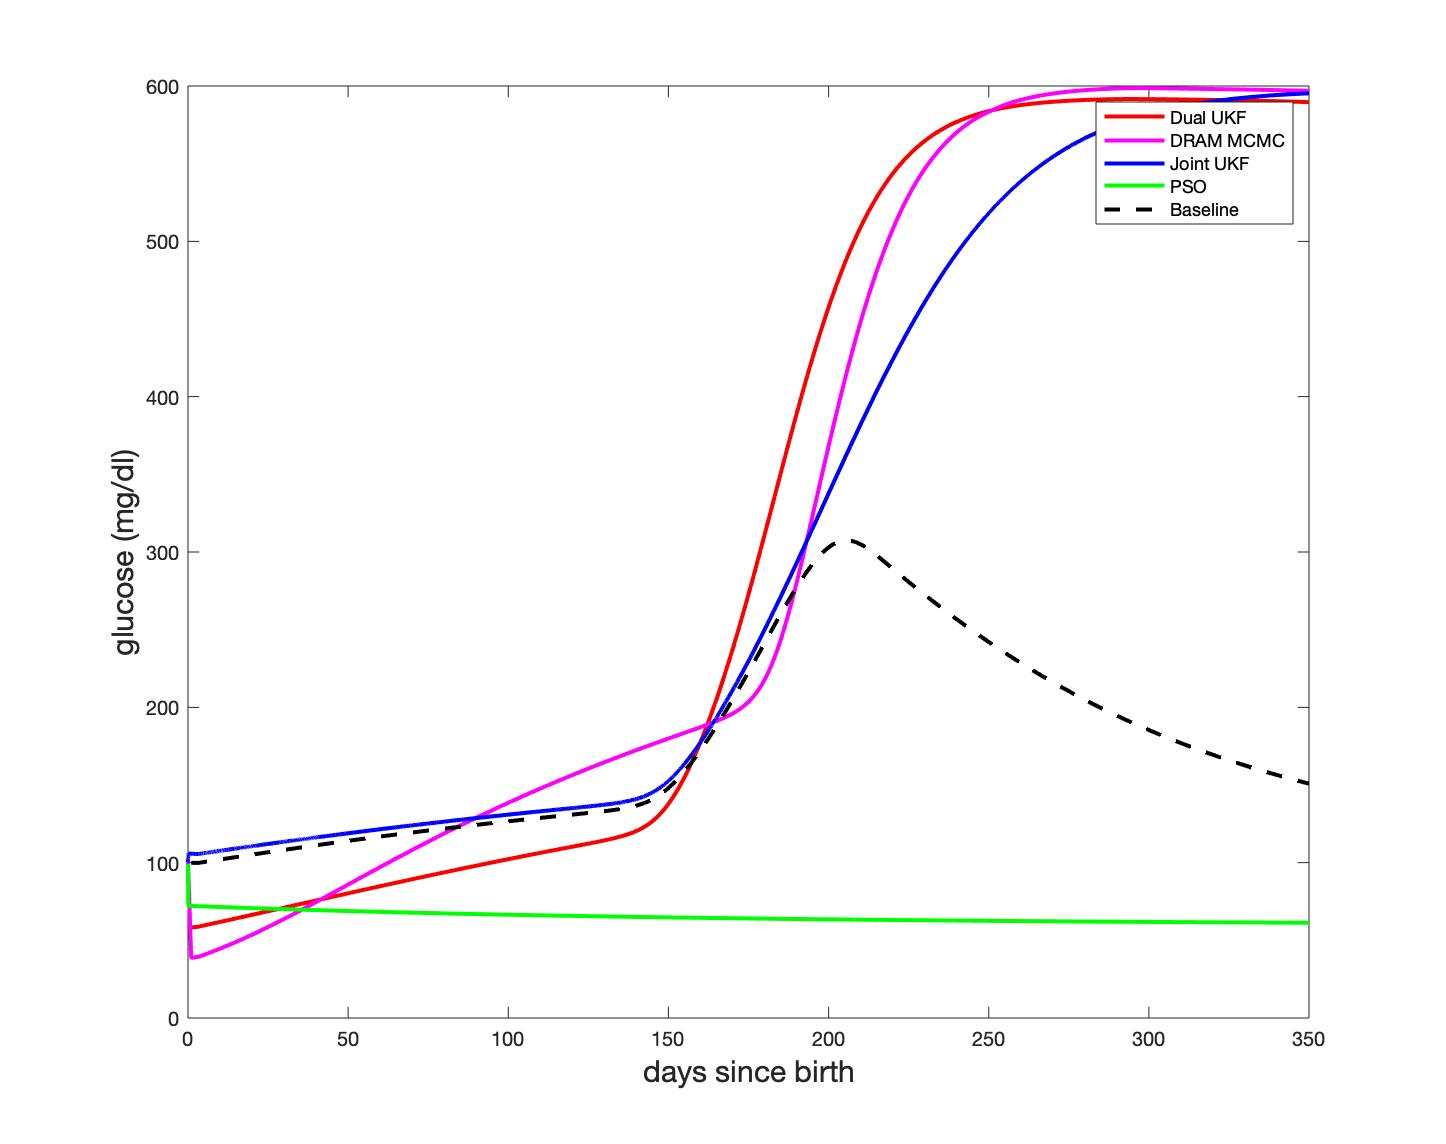
\includegraphics[width=15cm]{Kalman_Filter_Images/NoWave_Glucose_Comparisons.jpg}
    \caption{Glucose simulations using parameter values obtained from each parametrization algorithm and the baseline parameters, shown in black. The parameters from DRAM MCMC, Dual UKF, and Joint UKF each produce simulations where the NOD mouse still gets sick when no wave is present. On the other hand, the PSO parameters result in a healthy mouse, but the trajectory still does not fit our biological intuition, which is that of the Glucose under baseline values.}
    \label{fig:T1D_GlucoseAllAlgos_NoWave}
\end{figure}

Unfortunately, none of our algorithms are able to capture the behavior of an NOD mouse with no wave where the mouse has a slight increase in Glucose levels before returning to a healthy state, which is shown by the black dashed line. However, we see two different incorrect behaviors here. Using the Dual UKF, Joint UKf, and DRAM MCMC parameters the Glucose trajectory reaches a sick steady state, much like we have seen throughout this paper. However, interestingly with the PSO parameters, the Glucose never makes an initial rise whatsoever and remains at the healthy state. It will be very important moving forward to understand the issues and differences between these results in hopes of finding parameters that pass this crucial biological check.